\documentclass{standalone}
\usepackage{tikz}
\usetikzlibrary{patterns, positioning}

\begin{document}
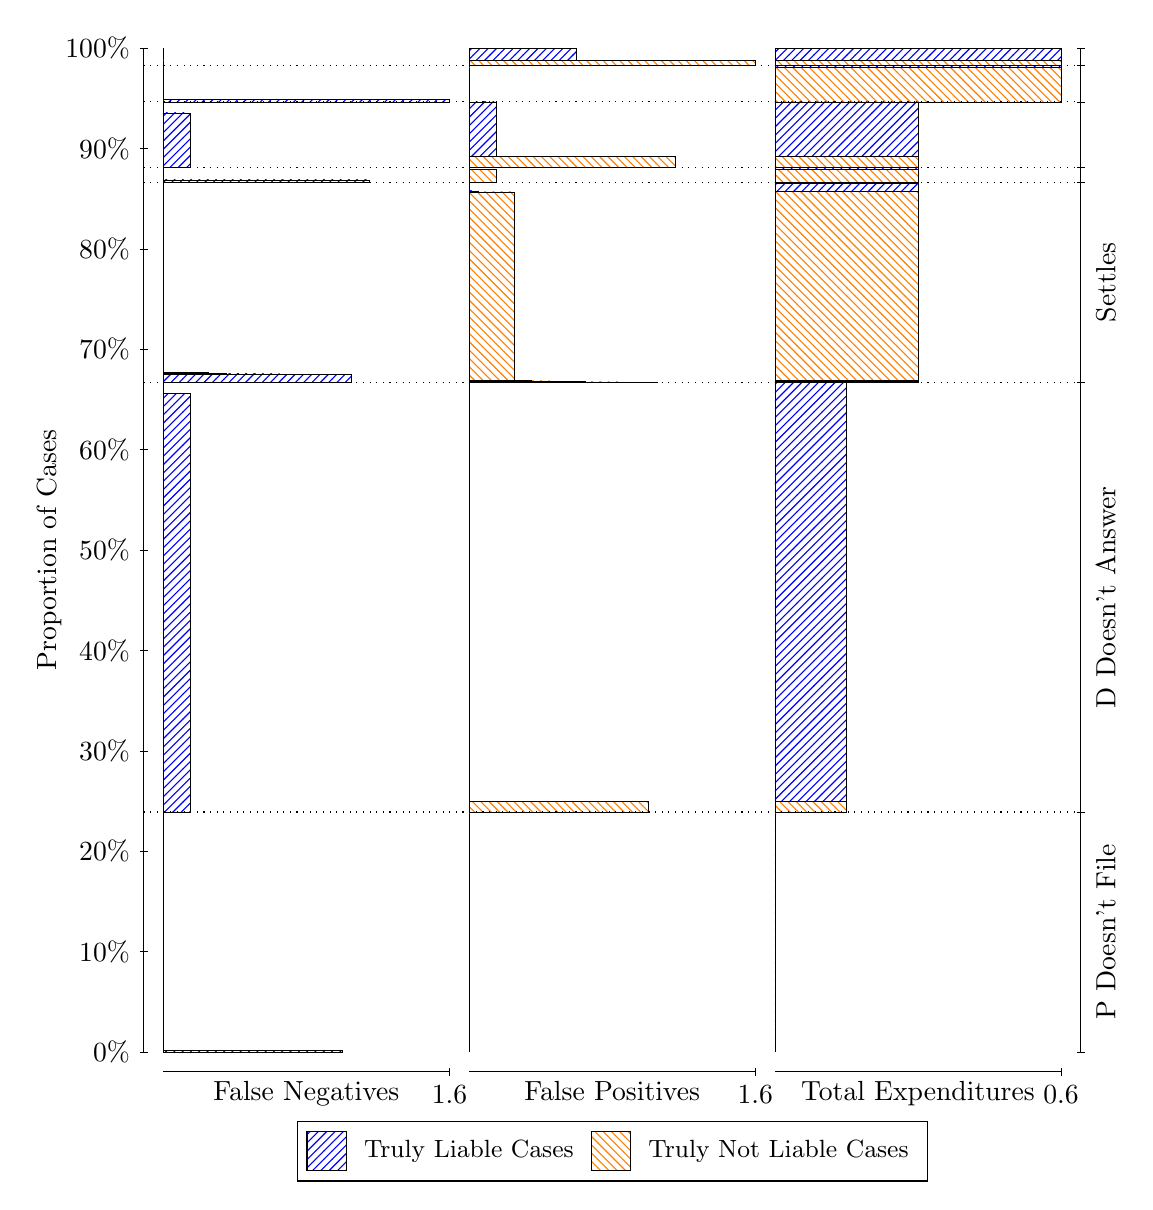
\begin{tikzpicture}
\draw[black, very thin] (1.5,1.75) -- (1.5,14.5);
\node[rotate=90, anchor=center] at (0.3, 8.125) {Proportion of Cases};
\draw[black, very thin] (1.45,1.75) -- (1.55,1.75);
\node[anchor=east] at (1.45, 1.75) {0\%};
\draw[black, very thin] (1.45,3.025) -- (1.55,3.025);
\node[anchor=east] at (1.45, 3.025) {10\%};
\draw[black, very thin] (1.45,4.3) -- (1.55,4.3);
\node[anchor=east] at (1.45, 4.3) {20\%};
\draw[black, very thin] (1.45,5.575) -- (1.55,5.575);
\node[anchor=east] at (1.45, 5.575) {30\%};
\draw[black, very thin] (1.45,6.85) -- (1.55,6.85);
\node[anchor=east] at (1.45, 6.85) {40\%};
\draw[black, very thin] (1.45,8.125) -- (1.55,8.125);
\node[anchor=east] at (1.45, 8.125) {50\%};
\draw[black, very thin] (1.45,9.4) -- (1.55,9.4);
\node[anchor=east] at (1.45, 9.4) {60\%};
\draw[black, very thin] (1.45,10.675) -- (1.55,10.675);
\node[anchor=east] at (1.45, 10.675) {70\%};
\draw[black, very thin] (1.45,11.95) -- (1.55,11.95);
\node[anchor=east] at (1.45, 11.95) {80\%};
\draw[black, very thin] (1.45,13.225) -- (1.55,13.225);
\node[anchor=east] at (1.45, 13.225) {90\%};
\draw[black, very thin] (1.45,14.5) -- (1.55,14.5);
\node[anchor=east] at (1.45, 14.5) {100\%};

\draw[black, very thin] (13.4,1.75) -- (13.4,14.5);
\draw[black, very thin] (13.35,1.75) -- (13.45,1.75);
\node[anchor=west] at (13.35, 1.75) {};
\draw[black, very thin] (13.35,4.7971) -- (13.45,4.7971);
\node[anchor=west] at (13.35, 4.7971) {};
\draw[black, very thin] (13.35,10.255) -- (13.45,10.255);
\node[anchor=west] at (13.35, 10.255) {};
\draw[black, very thin] (13.35,12.796) -- (13.45,12.796);
\node[anchor=west] at (13.35, 12.796) {};
\draw[black, very thin] (13.35,12.983) -- (13.45,12.983);
\node[anchor=west] at (13.35, 12.983) {};
\draw[black, very thin] (13.35,13.816) -- (13.45,13.816);
\node[anchor=west] at (13.35, 13.816) {};
\draw[black, very thin] (13.35,14.282) -- (13.45,14.282);
\node[anchor=west] at (13.35, 14.282) {};
\draw[black, very thin] (13.35,14.5) -- (13.45,14.5);
\node[anchor=west] at (13.35, 14.5) {};

\draw[black, very thin, pattern color=blue, pattern=north east lines] (1.75,1.75) rectangle (4.0208,1.7705);
\draw[black, very thin, pattern color=orange, pattern=north west lines] (1.75,1.7705) rectangle (1.75,4.7971);
\draw[black, very thin, pattern color=blue, pattern=north east lines] (1.75,4.7971) rectangle (2.0906,10.116);
\draw[black, very thin, pattern color=orange, pattern=north west lines] (1.75,10.116) rectangle (1.75,10.255);
\draw[black, very thin, pattern color=blue, pattern=north east lines] (1.75,10.255) rectangle (4.1344,10.357);
\draw[black, very thin, pattern color=blue, pattern=north east lines] (1.75,10.357) rectangle (3.9073,10.358);
\draw[black, very thin, pattern color=blue, pattern=north east lines] (1.75,10.358) rectangle (3.6802,10.359);
\draw[black, very thin, pattern color=blue, pattern=north east lines] (1.75,10.359) rectangle (3.4531,10.36);
\draw[black, very thin, pattern color=blue, pattern=north east lines] (1.75,10.36) rectangle (3.226,10.362);
\draw[black, very thin, pattern color=blue, pattern=north east lines] (1.75,10.362) rectangle (2.999,10.363);
\draw[black, very thin, pattern color=blue, pattern=north east lines] (1.75,10.363) rectangle (2.7719,10.363);
\draw[black, very thin, pattern color=blue, pattern=north east lines] (1.75,10.363) rectangle (2.5448,10.364);
\draw[black, very thin, pattern color=blue, pattern=north east lines] (1.75,10.364) rectangle (2.3177,10.378);
\draw[black, very thin, pattern color=orange, pattern=north west lines] (1.75,10.378) rectangle (1.75,12.796);
\draw[black, very thin, pattern color=blue, pattern=north east lines] (1.75,12.796) rectangle (4.3615,12.824);
\draw[black, very thin, pattern color=orange, pattern=north west lines] (1.75,12.824) rectangle (1.75,12.983);
\draw[black, very thin, pattern color=blue, pattern=north east lines] (1.75,12.983) rectangle (2.0906,13.675);
\draw[black, very thin, pattern color=orange, pattern=north west lines] (1.75,13.675) rectangle (1.75,13.816);
\draw[black, very thin, pattern color=blue, pattern=north east lines] (1.75,13.816) rectangle (5.3833,13.848);
\draw[black, very thin, pattern color=orange, pattern=north west lines] (1.75,13.848) rectangle (1.75,14.282);
\draw[black, very thin, pattern color=orange, pattern=north west lines] (1.75,14.282) rectangle (1.75,14.34);
\draw[black, very thin, pattern color=blue, pattern=north east lines] (1.75,14.34) rectangle (1.75,14.5);
\draw[black, very thin, pattern color=orange, pattern=north west lines] (5.6333,1.75) rectangle (5.6333,4.7766);
\draw[black, very thin, pattern color=blue, pattern=north east lines] (5.6333,4.7766) rectangle (5.6333,4.7971);
\draw[black, very thin, pattern color=orange, pattern=north west lines] (5.6333,4.7971) rectangle (7.9042,4.9363);
\draw[black, very thin, pattern color=blue, pattern=north east lines] (5.6333,4.9363) rectangle (5.6333,10.255);
\draw[black, very thin, pattern color=orange, pattern=north west lines] (5.6333,10.255) rectangle (8.0177,10.258);
\draw[black, very thin, pattern color=orange, pattern=north west lines] (5.6333,10.258) rectangle (7.7906,10.258);
\draw[black, very thin, pattern color=orange, pattern=north west lines] (5.6333,10.258) rectangle (7.5635,10.259);
\draw[black, very thin, pattern color=orange, pattern=north west lines] (5.6333,10.259) rectangle (7.3365,10.259);
\draw[black, very thin, pattern color=orange, pattern=north west lines] (5.6333,10.259) rectangle (7.1094,10.266);
\draw[black, very thin, pattern color=orange, pattern=north west lines] (5.6333,10.266) rectangle (6.8823,10.266);
\draw[black, very thin, pattern color=orange, pattern=north west lines] (5.6333,10.266) rectangle (6.8823,10.27);
\draw[black, very thin, pattern color=orange, pattern=north west lines] (5.6333,10.27) rectangle (6.6552,10.273);
\draw[black, very thin, pattern color=orange, pattern=north west lines] (5.6333,10.273) rectangle (6.4281,10.277);
\draw[black, very thin, pattern color=orange, pattern=north west lines] (5.6333,10.277) rectangle (6.201,12.673);
\draw[black, very thin, pattern color=blue, pattern=north east lines] (5.6333,12.673) rectangle (5.7469,12.687);
\draw[black, very thin, pattern color=blue, pattern=north east lines] (5.6333,12.687) rectangle (5.6333,12.796);
\draw[black, very thin, pattern color=orange, pattern=north west lines] (5.6333,12.796) rectangle (5.974,12.955);
\draw[black, very thin, pattern color=blue, pattern=north east lines] (5.6333,12.955) rectangle (5.6333,12.983);
\draw[black, very thin, pattern color=orange, pattern=north west lines] (5.6333,12.983) rectangle (8.2448,13.123);
\draw[black, very thin, pattern color=blue, pattern=north east lines] (5.6333,13.123) rectangle (5.974,13.816);
\draw[black, very thin, pattern color=orange, pattern=north west lines] (5.6333,13.816) rectangle (5.6333,14.25);
\draw[black, very thin, pattern color=blue, pattern=north east lines] (5.6333,14.25) rectangle (5.6333,14.282);
\draw[black, very thin, pattern color=orange, pattern=north west lines] (5.6333,14.282) rectangle (9.2667,14.34);
\draw[black, very thin, pattern color=blue, pattern=north east lines] (5.6333,14.34) rectangle (6.9958,14.5);
\draw[black, very thin, pattern color=orange, pattern=north west lines] (9.5167,1.75) rectangle (9.5167,4.7766);
\draw[black, very thin, pattern color=blue, pattern=north east lines] (9.5167,4.7766) rectangle (9.5167,4.7971);
\draw[black, very thin, pattern color=orange, pattern=north west lines] (9.5167,4.7971) rectangle (10.425,4.9363);
\draw[black, very thin, pattern color=blue, pattern=north east lines] (9.5167,4.9363) rectangle (10.425,10.255);
\draw[black, very thin, pattern color=orange, pattern=north west lines] (9.5167,10.255) rectangle (11.333,10.266);
\draw[black, very thin, pattern color=blue, pattern=north east lines] (9.5167,10.266) rectangle (11.333,10.284);
\draw[black, very thin, pattern color=orange, pattern=north west lines] (9.5167,10.284) rectangle (11.333,12.68);
\draw[black, very thin, pattern color=blue, pattern=north east lines] (9.5167,12.68) rectangle (11.333,12.783);
\draw[black, very thin, pattern color=orange, pattern=north west lines] (9.5167,12.783) rectangle (11.333,12.793);
\draw[black, very thin, pattern color=blue, pattern=north east lines] (9.5167,12.793) rectangle (11.333,12.796);
\draw[black, very thin, pattern color=orange, pattern=north west lines] (9.5167,12.796) rectangle (11.333,12.955);
\draw[black, very thin, pattern color=blue, pattern=north east lines] (9.5167,12.955) rectangle (11.333,12.983);
\draw[black, very thin, pattern color=orange, pattern=north west lines] (9.5167,12.983) rectangle (11.333,13.123);
\draw[black, very thin, pattern color=blue, pattern=north east lines] (9.5167,13.123) rectangle (11.333,13.816);
\draw[black, very thin, pattern color=orange, pattern=north west lines] (9.5167,13.816) rectangle (13.15,14.25);
\draw[black, very thin, pattern color=blue, pattern=north east lines] (9.5167,14.25) rectangle (13.15,14.282);
\draw[black, very thin, pattern color=orange, pattern=north west lines] (9.5167,14.282) rectangle (13.15,14.34);
\draw[black, very thin, pattern color=blue, pattern=north east lines] (9.5167,14.34) rectangle (13.15,14.5);
\draw[black, dotted] (1.5,4.7971) -- (13.4,4.7971);
\draw[black, dotted] (1.5,10.255) -- (13.4,10.255);
\draw[black, dotted] (1.5,12.796) -- (13.4,12.796);
\draw[black, dotted] (1.5,12.983) -- (13.4,12.983);
\draw[black, dotted] (1.5,13.816) -- (13.4,13.816);
\draw[black, dotted] (1.5,14.282) -- (13.4,14.282);
\draw[black, very thin] (1.75,1.5) -- (5.3833,1.5);
\node[anchor=north] at (3.5667, 1.5) {False Negatives};
\draw[black, very thin] (5.3833,1.45) -- (5.3833,1.55);
\node[anchor=north] at (5.3833, 1.45) {1.6};

\draw[black, very thin] (5.6333,1.5) -- (9.2667,1.5);
\node[anchor=north] at (7.45, 1.5) {False Positives};
\draw[black, very thin] (9.2667,1.45) -- (9.2667,1.55);
\node[anchor=north] at (9.2667, 1.45) {1.6};

\draw[black, very thin] (9.5167,1.5) -- (13.15,1.5);
\node[anchor=north] at (11.333, 1.5) {Total Expenditures};
\draw[black, very thin] (13.15,1.45) -- (13.15,1.55);
\node[anchor=north] at (13.15, 1.45) {0.6};

\node[black, centered, rotate=90] at (13.72, 3.2736) {P Doesn't File};
\node[black, centered, rotate=90] at (13.72, 7.5261) {D Doesn't Answer};
\node[black, centered, rotate=90] at (13.72, 11.525) {Settles};





\draw (7.449999999999999,1.5) node[draw=none] (baseCoordinate) {};
\begin{scope}[align=center]
        \matrix[scale=0.5, draw=black, below=0.5cm of baseCoordinate, nodes={draw}, column sep=0.1cm]{
            \node[rectangle, draw, minimum width=0.5cm, minimum height=0.5cm, pattern=north east lines, pattern color=blue] {}; &
            \node[draw=none, font=\small] (B) {Truly Liable Cases}; &
            \node[rectangle, draw, minimum width=0.5cm, minimum height=0.5cm, pattern=north west lines, pattern color=orange] {}; &
            \node[draw=none, font=\small] (B) {Truly Not Liable Cases}; \\
            };
\end{scope}

\end{tikzpicture}
\end{document}